% =====================================================================
%  §3. Материальные поправки: Друде и рассеяние ν^γ
%
%  ЖАНР (STYLE.md): учебная литература. Ни путей, ни имён программ, ни
%  номеров гипотез. Прослеживаемость — ключи \srckey{3.x} и приложение.
%
%  Содержательная основа: BRIEF_FOR_D_teaching_ladder.md §4; SYNTHESIS.md
%  §4-5 (реестр гипотез HN5/HN11 с ΔAIC).
% =====================================================================
\section{Материальные поправки: Друде и рассеяние \texorpdfstring{$\nu^\gamma$}{nu\^{}gamma}}
\label{sec:drude}
\markboth{§\thesection. Друде и рассеяние}{}

Модель §\ref{sec:blanco} считала провод \textbf{идеально проводящим}: вся его роль сводилась к
геометрии, а вещественная часть импеданса появлялась только за счёт эванесцентных дифракционных
порядков (и в нашей полосе частот она равна нулю). Настоящий провод сделан из настоящего металла
с конечной проводимостью, и это добавляет два независимых физических эффекта, которые нужно
внести в модель \emph{поверх} геометрии Бланко. Этот параграф вводит оба и заканчивается уроком,
который пригодится для всей оставшейся части курса: улучшение согласия с данными и измеримость
параметра, отвечающего за это улучшение,~--- разные вещи.

\begin{tcolorbox}[enhanced,colback=cPanel,colframe=cGrid,boxrule=0.8pt,arc=2pt,
                  title={\bfseries\color{cAccent} Пререквизиты},coltitle=cAccent,
                  attach boxed title to top left={xshift=6pt,yshift=-2pt},
                  boxed title style={colback=cPanel,boxrule=0pt,arc=0pt},top=10pt]
\textbf{Нужно знать:} §\ref{sec:blanco} (эквивалентная схема, реактивные импедансы, откуда
берутся $\tperp,\tpar$); комплексный импеданс; понятие проводимости металла.\\[0.3em]
\textbf{Знать НЕ нужно:} микроскопическую теорию электронного транспорта. Модель Друде вводится
здесь на уровне одной формулы для поверхностного импеданса, без вывода из кинетического
уравнения.
\end{tcolorbox}

% ---------------------------------------------------------------------
\subsection{Конечная проводимость: поверхностный импеданс металла}
\label{subsec:drude-impedance}

\begin{intuition}
Идеальный проводник экранирует поле мгновенно и без потерь: поверхностный ток течёт строго по
поверхности, вглубь ничего не проникает. Настоящий металл~--- не идеальный проводник: поле
проникает на конечную глубину (скин-слой), там совершает работу над электронами, и часть энергии
уходит в тепло. С точки зрения внешней волны это выглядит как \emph{малый} дополнительный
импеданс на поверхности провода~--- не ноль, но и не большая величина, потому что металл всё же
хороший проводник на терагерцовых частотах.
\end{intuition}

\noindent
\term{Модель Друде} описывает проводимость металла как отклик свободных электронов с временем
релаксации $\tau_e$ (среднее время между столкновениями электрона с решёткой):
\begin{equation}
  \sigma(\omega)=\frac{\sigma_0}{1-\jj\omega\tau_e},
  \qquad
  Z_s(\omega)=\sqrt{\frac{\jj\omega\mu_0}{\sigma(\omega)}},
  \label{eq:drude}
\end{equation}
где $\sigma_0$~--- проводимость на постоянном токе, $\mu_0$~--- магнитная проницаемость вакуума,
$Z_s$~--- \term{поверхностный импеданс}, нормируемый на импеданс вакуума $Z_0$. Эта величина
входит в эквивалентную схему §\ref{sec:blanco} как малая добавка к реактивным импедансам
$Z_a,\ldots,Z_d$~--- на тех же местах, где раньше стоял чистый ноль.

\begin{strict}[: почему добавка малая и почему она комплексная]
На терагерцовых частотах $\omega\tau_e\ll1$ для типичных металлов ($\tau_e$~--- порядка
$10^{-14}$~с), поэтому $\sigma(\omega)\approx\sigma_0$ почти вещественна, а
$Z_s\propto\sqrt{\omega/\sigma_0}$~--- мала и растёт с частотой. Комплексность $Z_s$ означает, что
добавка вносит не только затухание (вещественная часть~--- омические потери, то, чего не было в
идеальном проводнике §2), но и малый дополнительный фазовый сдвиг (мнимая часть). Оба эффекта
одного порядка малости и одного физического происхождения~--- конечная проводимость,~--- поэтому
вводятся одной формулой, а не двумя независимыми поправками.
\end{strict}

\begin{warning}[: это не то же самое, что просачивание из §1]
Поправка Друде действует \textbf{одинаково на оба канала}~--- она модифицирует геометрическую
схему §2 целиком, а не создаёт новый путь для поля. Просачивание $\tpar$ (§\ref{subsec:leakage})
существовало бы даже для идеально проводящего провода~--- оно геометрическое, от неполноты
экранирования узкой решёткой. Друде добавляет к обоим каналам небольшую частотно-зависимую
поправку сверху, не создавая канал заново.
\end{warning}

% ---------------------------------------------------------------------
\subsection{Степенное рассеяние: феноменологический член потерь}
\label{subsec:power-law}

Поправка Друде объясняет часть отклонений от идеального проводника, но не все: после её включения
в модели остаётся систематический, гладкий по частоте остаток~--- амплитуда прошедшего поля падает
с частотой чуть быстрее или медленнее, чем предсказывает \eqref{eq:drude}. Стандартный приём~---
добавить \term{феноменологический} множитель потерь, не привязанный к конкретному микроскопическому
механизму:
\begin{equation}
  a_{\text{потери}}(\nu)=\exp\!\Big[-\tfrac12\,\tfrac{L}{4{,}343}\,\nu^{\gamma}\Big],
  \label{eq:power-law-loss}
\end{equation}
где $L$~--- амплитудный коэффициент потерь (во сколько децибел на единицу частотной шкалы), а
$\gamma$~--- показатель степени. Множитель $1/4{,}343=\ln10/10$ переводит децибелы в натуральный
показатель экспоненты.

\begin{intuition}
Классическое рэлеевское рассеяние на неоднородностях масштаба меньше длины волны даёт $\gamma=2$
(квадратичный рост потерь с частотой)~--- это своего рода <<умолчание>>, если механизм потерь не
уточняется. Но реальные механизмы (рассеяние на границах зёрен металла, эффект Фукса--Зондхаймера
в тонких проводящих слоях и другие) дают показатели, отличные от двух, причём часто дробные. Вместо
того чтобы выбирать один механизм заранее, формула~\eqref{eq:power-law-loss} оставляет $\gamma$
свободным параметром и позволяет данным сказать, какой показатель им нужен.
\end{intuition}

% ---------------------------------------------------------------------
\begin{figure}[t]
  \centering
  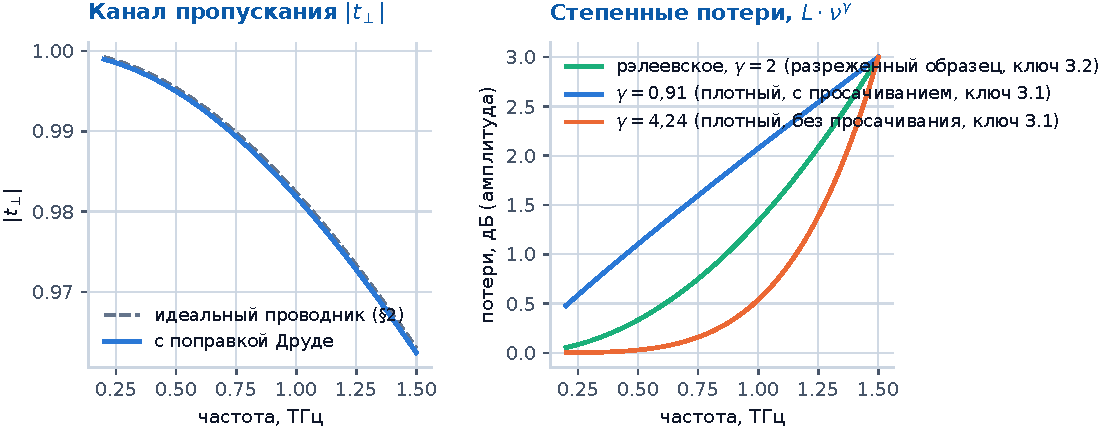
\includegraphics[width=\linewidth]{figures/fig03_drude.pdf}
  \caption{Модельный расчёт. Слева: канал пропускания с поправкой Друде и без неё (формула
  §\ref{subsec:drude-impedance} поверх геометрии §2, $D/P=0{,}56$)~--- отличие на рабочей полосе
  составляет тысячные доли и на глаз не заметно. Справа: множитель степенных потерь
  \eqref{eq:power-law-loss} для трёх показателей~$\gamma$, включая два значения из
  примера~\ref{subsec:no-measurement} (одна и та же величина потерь на верхней границе полосы,
  разный ход по частоте).}
  \label{fig:drude}
\end{figure}

% ---------------------------------------------------------------------
\subsection{«Эффект есть — параметр не измерен»}
\label{subsec:no-measurement}

Добавление члена~\eqref{eq:power-law-loss} к модели §2$+$Друде реально и заметно улучшает
согласие с данными. Возникает естественный вопрос: раз модель стала лучше, значит ли это, что мы
\emph{измерили} показатель рассеяния~$\gamma$? Ответ~--- поучительное <<нет>>, и разбор того, почему
именно нет, стоит того, чтобы задержаться.

\begin{example}[: улучшение согласия реально]\srckey{3.1}
На плотной решётке ($D/P=0{,}71$) добавление степенного члена потерь улучшает информационный
критерий на $\dAIC\approx-733$ относительно модели без него (шкала $\dAIC$ разбирается в §8;
здесь достаточно знать, что такая величина~--- уверенное, не случайное улучшение). Эффект
проверен и признан реальным.
\end{example}

\begin{warning}[: но сам показатель $\gamma$ плывёт]
На тех же данных значение $\gamma$ существенно зависит от того, включена ли в модель одновременно
явная поправка на просачивание (§\ref{subsec:leakage}, будет формально введена в модель в §6):
с учётом просачивания $\gamma\approx0{,}91$, без него~--- $\gamma\approx4{,}24$. Это не опечатка и
не ошибка подгонки~--- это \emph{один и тот же} набор данных, дающий вчетверо-впятеро разные оценки
одного и того же параметра в зависимости от соседнего слагаемого модели.
\end{warning}

\begin{intuition}[: почему так происходит]
Оба члена~--- степенные потери и просачивание~--- на верхних частотах рабочей полосы производят
похожий на вид эффект: плавный дополнительный спад амплитуды с частотой в канале подавления. Когда
в модели нет явного просачивания, показателю~$\gamma$ приходится \emph{за двоих} воспроизводить
форму спада, которая на самом деле частично принадлежит другому физическому механизму. Показатель
степени становится <<мусорной корзиной>>: он подстраивается под любую гладкую форму спада, доступную
модели, независимо от того, какой физический процесс её на самом деле создал.
\end{intuition}

\begin{example}[: на разреженном образце показатель ведёт себя иначе]\srckey{3.2}
На самом разреженном из образцов, где просачивание слабее выражено (§\ref{sec:electrodynamics}),
показатель определяется гораздо увереннее~--- $\gamma\approx2{,}04$ с узким интервалом
$[1{,}96;\,2{,}15]$~--- и близок к классическому рэлеевскому значению~$2$. Проверка того, общий ли
это показатель для всех образцов (единая материальная константа, не зависящая от конкретной
решётки), пока не подтверждена: слишком мало образцов дают устойчивую оценку, чтобы делать вывод
об универсальности.
\end{example}

\begin{tcolorbox}[enhanced,colback=cS1!7,colframe=cS1,boxrule=0pt,leftrule=3pt,arc=1pt]
\textbf{Различение, которое стоит запомнить на весь курс.} \emph{«Модель с этим членом лучше
описывает данные»} и \emph{«численное значение этого параметра надёжно»} — два разных
утверждения, и первое не влечёт второго. Эффект существует и достоверен ($\dAIC=-733$); конкретное
число, которым модель его описывает, зависит от того, что ещё присутствует в модели рядом, и может
меняться в разы. Курс вернётся к этому различению как к общему методическому правилу в §8--§9 и как
к готовому рабочему принципу в §10.
\end{tcolorbox}

% ---------------------------------------------------------------------
\subsection{Типичные ошибки этого параграфа}

\begin{enumerate}[leftmargin=1.6em,itemsep=0.25em]
  \item Считать поправку Друде источником просачивания. Это независимые эффекты: Друде~---
        конечная проводимость, действует на оба канала одинаково; просачивание~--- геометрическая
        неполнота экранирования, создаёт новый путь для поля (§\ref{subsec:drude-impedance}).
  \item Принять улучшение $\dAIC$ от степенного члена потерь за измерение показателя~$\gamma$.
        Улучшение согласия и определённость параметра, отвечающего за него,~--- разные вопросы
        (§\ref{subsec:no-measurement}).
  \item Забыть проверить, с чем ещё в модели конкурирует новый параметр, прежде чем доверять его
        числовому значению. Оценка $\gamma$ вчетверо меняется от присутствия соседнего члена
        модели.
  \item Обобщать оценку показателя рассеяния с одного образца на все остальные без проверки: пока
        это не подтверждено.
\end{enumerate}

\clearpage
